\section{approach}\label{sec:approach}

As explained in~\autoref{sec:background}, Curdleproofs makes use of three different proofs.
This work focuses on improving the underlying~\gls{ipa}.
Especially the running time and proof size of the protocol are of interest.
The following is our approach to, how we modified the~\gls{ipa}.

\subsection{Springproofs}\label{sec:approach-springproofs}
In Chapter 6 of Curdleproofs~\cite{Curdleproofs}, they explain the efficiency of the protocol, including also the size of the proof.
They specifically mention that the proof has size $18+10 \log(\ell+4)\mathbb{G}$, $7\mathbb{F}$.
As the proof size is dependent on the size of the shuffle, $\ell$, an interest in the possibility of reducing this parameter arises.
The current proposal of curdleproofs only works on shuffles, where the size is a power of 2.
The reason is that the underlying proofs, such as the~\gls{ipa}, needs to fold recursively down to 1, by halving the size in every round.

The Springproofs protocol~\cite{zhang2024springproofs} can be used very effectively in this scenario.
The theory of Springproofs provides support for~\glspl{ipa} to use vectors of arbitrary length.
Using the findings of Springproofs means Curdleproofs could be used on shuffle sizes other than powers of two.
As such, they could lower the shuffle size from the current 128 to a size significantly lower, given it is still secure.
Seeing the proof size of Curdleproofs being dependent on $\ell$ means that this modification would greatly help in lowering it.

One of the most notable findings in Springproofs is the usage of their so-called scheme function.
This function is used to ensure that the~\gls{ipa} eventually will fold down to a vector of size 1.
In a general~\gls{ipa}, Curdleproofs included, if the size of the vectors were not a power of two, the argument would not recursive down to size 1, as they work by halving the vectors every recursive round.


The core concept of the Springproofs scheme function is to split the vectors into sets, $T,S$ before each recursive round of the protocol.
Then, the fold for that round is only done on one of the two sets, $T$, before the other set, $S$, is appended again at the end of the recursive round.

Springproofs present different scheme functions and prove some of them to be optimal.
One of these optimal functions is an optimized version of their \textit{pre-compression method}, which splits the vectors as seen in~\autoref{fig:schemefunc}.
The computation is for finding the set, $T$.

\begin{figure}[ht]
\begin{framed}
    \begin{lstlisting}[language=Python,mathescape=true,label={lst:schemefunc}]
    input: $n$, where $n>0$

    $\{n\}\gets n$
    $N\gets 2^{\lceil\log n\rceil-1}$
    $i_h \gets \lfloor (2N-n)/2\rfloor+1$
    $i_t=\lfloor n/2\rfloor$
    if $n\neq N$:
        $\{T\}\gets(i_h:i_t)\cup(N+1:n)$
    else if $n=N$:
        $\{T\}\gets(1:n)$
    $\{S\}\gets\{n\}-\{T\}$
    \end{lstlisting}
\end{framed}
\caption{Scheme function \textbf{\textit{f}} used in CAAUrdleproofs}
\label{fig:schemefunc}
\end{figure}

This can also visually be seen in~\autoref{fig:fold}(b), which is figure 1 of the Springproofs paper~\cite{zhang2024springproofs}.
In \autoref{fig:fold}(a) is a scheme function which simply pads the vector to the next power of two before running an~\gls{ipa}.
If one wanted to run current~\glspl{ipa}s on vector that are not a power of two, this would generally be the easiest way to achieve that.
Though, this defeats the attempt of lowering the proof size, as it would now correspond to running an~\gls{ipa} on the size of the next power of two.

\begin{figure*}[t]
    \centering
    \subfloat[\centering Padding Method]{{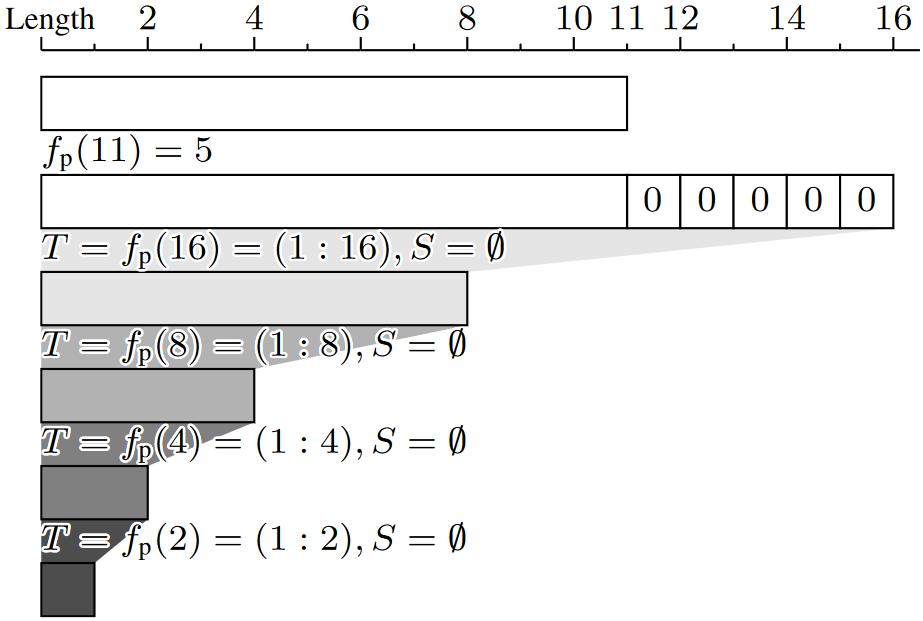
\includegraphics[width=0.43\textwidth]{figures/padding} }}%
    \qquad
    \subfloat[\centering Optimal Pre-Compression Method]{{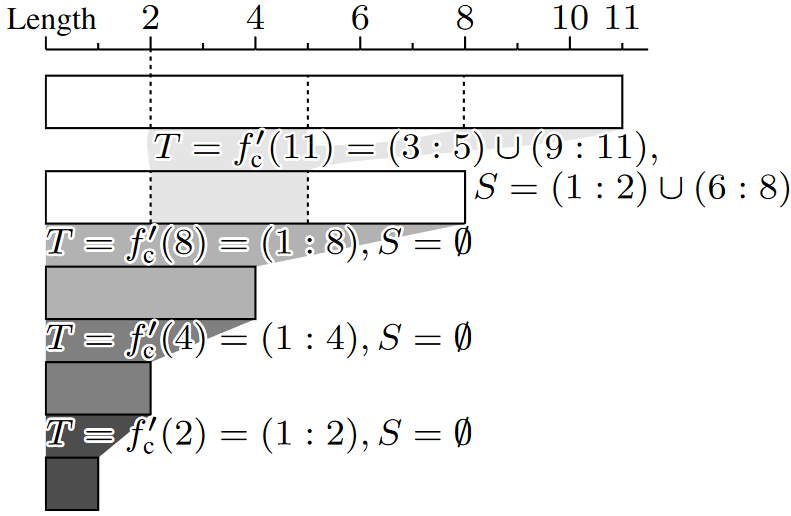
\includegraphics[width=0.45\textwidth]{figures/fold} }}%
    \caption{Folding visualization as seen in the Springproofs paper}%
    \label{fig:fold}%
\end{figure*}

It is notable to mention that using the folding as shown in~\autoref{fig:fold}(b) results in the second recursive round being a size corresponding to a power of two.
This means that the rest of the protocol will run as a general~\gls{ipa}, without the actual need for splitting the vectors, which can also be seen in~\autoref{fig:schemefunc}.

With the idea from Springproofs in mind, we have made a modification to the~\gls{ipa} of Curdleproofs
We call this modified protocol, CAAUrdleproof.
For generality and readability, we show the split of vectors happening every round.

First of all, we have the prover computation, where the proof is constructed.
The construction can be seen in~\autoref{fig:ipa-prover}.

\begin{figure}[h]
\begin{framed}
    \begin{lstlisting}[language=Python,mathescape=true,label={lst:ipa-prover}]
$\textbf{Step 1:}$
$\textbf{r}_C,\textbf{r}_D\overset{\$}{\leftarrow}\mathbb{F}^n$
 where $(\textbf{r}_C\times \textbf{d} + \textbf{r}_D\times \textbf{c})=0\text{ and }\textbf{r}_C\times \textbf{r}_D=0$
$B_C\gets \textbf{r}_C\times \textbf{G}$
$B_D\gets \textbf{r}_D\times \textbf{G}'$
$\alpha,\beta\gets$Hash$(C,D,z,B_C,B_C)$
$\textbf{c}\gets \textbf{r}_C+\alpha \textbf{c}$
$\textbf{d}\gets \textbf{r}_D+\alpha \textbf{d}$
$H\gets\beta H$
$\textbf{Step 2:}$
$m\gets n$
while $1\leq j\leq\lceil \log m\rceil:$
    $T,S\gets \textbf{\textit{f(}}n\textbf{\textit{)}}$
    $n\gets \frac{|T|}{2}$
    $\textbf{c}=\textbf{c}_T$, $\textbf{cS}=\textbf{c}_S$
    $\textbf{d}=\textbf{d}_T$, $\textbf{dS}=\textbf{d}_S$
    $\textbf{G}=\textbf{G}_T$, $\textbf{GS}=\textbf{G}_S$
    $\textbf{G}'=\textbf{G}'_T$, $\textbf{GS}'=\textbf{G}'_T$
    $L_{C,j}\gets\textbf{c}_{[:n]}\times\textbf{G}_{[n:]}+(\textbf{c}_{[:n]}\times\textbf{d}_{[n:]})H$
    $L_{D,j}\gets\textbf{d}_{[n:]}\times\textbf{G}'_{[:n]}$
    $R_{C,j}\gets\textbf{c}_{[n:]}\times\textbf{G}_{[:n]}+(\textbf{c}_{[n:]}\times\textbf{d}_{[:n]})H$
    $R_{D,j}\gets\textbf{d}_{[:n]}\times\textbf{G}'_{[n:]}$
    $\pi_j\gets(L_{C,j},L_{D,j},R_{C,j},R_{D,j})$
    $\gamma_j\gets Hash(\pi_j)$
    $\textbf{c}\gets\textbf{cS}\|\textbf{c}_{[:n]}+\gamma_j^{-1}\textbf{c}_{[n:]}$
    $\textbf{d}\gets\textbf{dS}\|\textbf{d}_{[:n]}+\gamma_j\textbf{d}_{[n:]}$
    $\textbf{G}\gets\textbf{GS}\|\textbf{G}_{[:n]}+\gamma_j\textbf{G}_{[n:]}$
    $\textbf{G}'\gets\textbf{GS}'\|\textbf{G}'_{[:n]}+\gamma_j^{-1}\textbf{G}'_{[n:]}$
    $n\gets len(c)$
$\textbf{Step 3:}$
$c\gets c_1$
$d\gets d_1$

return $(B_C,B_D,\mathbf{\pi},c,d)$
    \end{lstlisting}
\end{framed}
\caption{Prover computation for CAAU-IPA in CAAUrdleproofs}
\label{fig:ipa-prover}
\end{figure}

First, we have step 1, which is the setup phase.
It is done exactly the same way as in Curdleproofs.
To ensure zero-knowledge, two blinding vectors for each commitment are constructed.
These are also given the properties, $(\mathbf{r}_C\times \mathbf{d}+\mathbf{r}_D\times \mathbf{c})=0$ and $\mathbf{r}_C\times\mathbf{r}_D=0$, ensuring the completeness of the protocol.

From the public input, hash values $\alpha,\beta$ are then computed.
These are used to ensure the soundness of the protocol.

The two vectors are then blinded and multiplied by the $\alpha$ hash to ensure the zero-knowledge and soundness, as well as $H=\beta H$.


Now, the recursive proof construction begins.
As explained, at the start of the recursive round, the \texttt{while}-loop, we find the split of the vectors, with $f(n)$ being the function from~\autoref{fig:schemefunc}.
Then, we find half the length of the $T$ set, as this is the set, we are doing the recursive round on.
Equally we split our witness vectors and the group vectors using $T$ and $S$.

After this, the prover constructs cross commitment elements that are computed on the $T$ set.
These are added to the proof, which eventually is available to the verifier.
They are also used to construct a hash value, $\gamma_j$, in the next step.

This value is used for completing the folding of $\mathbf{c},\mathbf{d},\mathbf{G},\mathbf{G'}$.
We do the fold as in the original Curdleproofs protocol, while also appending the elements of $S$ back onto the vectors.
The figure shows a concatenation, but it is important to know that the vectors are appended together as shown in~\autoref{fig:fold}(b).

At last,~$n$ is updated to the length of the concatenated vectors before starting a new round.

The result of this is a proof constructed in $\lceil \log n \rceil$ rounds, but with the proof size being smaller than if the shuffle size was a power of 2.

The now constructed proof is then supposed to be added to the block in the chain at the given time slot~\cite{Whisk2024}.
Having the proof on the blockchain allows for each validator to asynchronously verify whether it is a valid proof.
Again, the originally proposed verifying protocol has been modified according to Springproofs, which is seen in~\autoref{fig:ipa-verifier}.

\begin{figure}[h]
\begin{framed}
\begin{lstlisting}[language=Python,mathescape=true,label={lst:ipa-verifier}]
$\textbf{Step 1:}$
$(\textbf{G},\textbf{G}',H)\gets$parse$(crs_{dl_{inner}})$
$(C,D,z)\gets$parse$(\phi_{dl_{inner}})$
$(B_C,B_D,\mathbf{\pi},c,d)\gets$parse$(\pi_{dl_{inner}})$
$\alpha,\beta\gets$Hash$(C,D,z,B_C,B_D)$
$H\gets \beta H$
$C\gets B_C+\alpha C+(\alpha^2z)H$
$D\gets B_D+\alpha D$

$\textbf{Step 2:}$
$m\gets \lceil\log n\rceil$
for $1\leq j\leq m$
    $T,S\gets \textbf{\textit{f(}}n\textbf{\textit{)}}$
    $n\gets \frac{|T|}{2}$
    $\textbf{G}=\textbf{G}_T$, $\textbf{GS}=\textbf{G}_S$
    $\textbf{G}'=\textbf{G}'_T$, $\textbf{GS}'=\textbf{G}'_T$
    $(L_{C,j},L_{D,j},R_{C,j},R_{D,j})\gets$parse$(\pi_j)$
    $\gamma_j\gets$Hash$(\pi_j)$
    $C\gets\gamma_j L_{C,j}+C+\gamma_j^{-1}R_{C,j}$
    $D\gets\gamma_j L_{D,j}+D+\gamma_j^{-1}R_{D,j}$
    $\textbf{G}\gets\textbf{GS}\|\textbf{G}_{[:n]}+\gamma_j\textbf{G}_{[n:]}$
    $\textbf{G}'\gets\textbf{GS}'\|\textbf{G}'_{[:n]}+\gamma_j^{-1}\textbf{G}'_{[n:]}$
    $n\gets\text{len}(\textbf{G})$

$\textbf{Step 3:}$
Check $C=c\times G_1+cdH$
Check $D=d\times G'_1$
$\text{return 1 if both checks pass, else return 0}$
\end{lstlisting}
\end{framed}
\caption{Verifier computation for CAAU-IPA in CAAUrdleproofs}
\label{fig:ipa-verifier}
\end{figure}

The changes to the verifier protocol are equivalent to the ones made to the prover protocol.
First, the vectors are divided into the two sets, $|T|,|S|$.
The verifier then retrieves the cross-product commitment update values, $L_{C,j},L_{D,j},R_{C,j},R_{D,j}$.
These are used for constructing a new commitment according to the fold made at round $i$.
The corresponding left and right side cross-product are multiplied by a challenge, $\gamma_j,\gamma_j^{-1}$, respectively.
By this time, the $C$ and $D$ commitments are a commitment to the original commitments along with the folded commitment.

$\mathbf{G,G'}$ are updated as in~\autoref{fig:ipa-prover} before the protocol updates $n$ to be the length of the newly constructed vectors.

As in the prover protocol, this is then repeated for $\log n$ round, after which the vectors have length $1$.

At the end of the protocol, the verifier now does its final check.
From the prover, it has retreived the folded down $c$ and $d$ vectors.
It therefore constructs commitments with these elements.
So, it constructs $c\times G_1+cdH$, which is the structure of the $C$ commitment as well as $d\times G'_1$, which is the structure of the $D$ commitment.
The verifier now checks if these commitments match the commitments that he constructed in the recursive protocol.
If so, the verifier accepts the proof.


\subsection{Shuffle security}\label{subsec:approach-shuffle-security}
The shuffle method proposed by Larsen et al.~\cite{cryptoeprint:2022/560} that was used in Curdleproofs is based on the idea of shuffling a list of proposers over a set of slots.
The shuffle itself, however, is not too complex.
A formal definition of the shuffle is given in~\autoref{fig:shuffle}~\cite{cryptoeprint:2022/560}.

\begin{figure}[ht]
\begin{framed}
    \[
        \Pi(c_1, \ldots, c_n)
    \]
    \rule{\linewidth}{0.4pt}

    \noindent
    \textbf{For} $t \in [T]$ \textbf{:}
    \begin{itemize}
        \item[$S_t$] picks random $\{i_1, \ldots, i_k\} \subset [n]$
        \item[$S_t$] computes $(\tilde{c}_{i_1}, \ldots, \tilde{c}_{i_k}) \leftarrow \text{Shuffle}(c_{i_1}, \ldots, c_{i_k})$
        \item[$S_t$] publishes $(\tilde{c}_{i_1}, \ldots, \tilde{c}_{i_k})$
    \end{itemize}
\end{framed}
\caption{Distributed shuffling protocol.}
\label{fig:shuffle}
\end{figure}

Here the set $(c_1, \ldots, c_n)$ is a set of ciphertexts that are shuffled over $T$ slots.
In each slot $t$, a subset of the ciphertexts ${i_1, \ldots, i_k}$ is chosen randomly, shuffled, and added back to the list of ciphertexts.
The shuffler then re-encrypts the ciphertexts and publishes them.
This process is repeated for $T$ slots and the shuffle is complete.
During the $T$ shuffles, some shufflers may be adversarial.
This means that whenever the shuffling process is taking place, a part of the shuffles may be adversarial, which can be seen as not being shuffled.
Therefore, the number of honest shuffles that happen during the shuffle process is $T_H = T - \alpha$, where $\alpha$ is the number of adversarial tracked ciphertexts.

The shuffle is secure if none of the following two events occur.
The first event is a short backtracking, where an adversary can find the original ciphertexts from the shuffled ciphertexts.
Since the subsets of ciphertexts are chosen randomly in each shuffle, if there are enough adversarial shufflers in a row to end the process, then a short backtracking is possible.

The second event that can occur is related to the fact that every shuffle distributes the possibility of a certain ciphertext to be in a certain slot.
So, if a shuffle contains a lot of ciphertexts with a larger than average chance of containing a certain ciphertext, then that would imply that there is a higher chance of that ciphertext being in that slot.

It is theoretically possible to find an optimal number of shuffles, given the shuffle size, and a number of adversarial shufflers, to guarantee that the shuffle is secure.
For any $0 < \delta < 1/3$, if $T \geq 20 n / k \ln(n/\delta) + \beta $ and $ k \geq 256 \ln^2(n/\delta)(1 - \alpha/n)^{-2}$.
If $T$ and $k$ are chosen such that the above two conditions are met, then the protocol is an $(\epsilon , \delta)$-secure $(T,n,k)$-shuffle in the presence of a $(\alpha, \beta)$-adversary where $\epsilon = 2/(n-\alpha)$.

This formula is the lowest theoretically proven bound for $T$ and $k$.
Plotting numbers relevant to Whisk will show that this theoretical bound is too large to use for argumentation of security.
It is, however, possible to find lower secure values for $T$ and $k$, but this has to be done experimentally.


\subsection{Implementation}\label{subsec:approach-implementation}
Implementing the above-explained CAAUrdleproofs protocol introduced some optimizations required to have the code run as fast as possible.
These are explained in the following with a focus on how CAAUrdleproofs differentiates itself from Curdleproofs.
Both our implementation of CAAUrdleproofs and the experiment involving the security of the shuffle are publicly available on GitHub~\footnote{\href{https://github.com/AAU-Dat/curdleproofsplus/tree/SIPA}{https://github.com/AAU-Dat/curdleproofsplus/tree/SIPA}}.
The implementation of CAAUrdleproofs is a fork of and builds directly on the already existing Curdleproofs code.
\subsubsection{CAAUdleproofs}
The protocol in Curdleproofs~\cite{Curdleproofs} introduces a lot of multiscalar multiplications.
As such, CAAUrdleproofs also introduces these multiplications.
This allows for checking calculations of the form:
\begin{align}
    C\stackrel{?}{=}\mathbf{x}\times(\mathbf{g}\|\mathbf{h}\|G_T\|G_U\|H\|\mathbf{R}\|\mathbf{S}\|\mathbf{T}\|\mathbf{U})
\end{align}
As explained by Curdleproofs, the verifier computation can be significantly optimized by checking the multiscalar multiplications as a single check at the end of the protocol instead.

CAAUrdleproofs introduced a slight difference on this topic in regard to the~\glspl{ipa}, \texttt{sameperm} and \texttt{same multiscalar}.
In each recursive round, both the folded vectors and the commitments are being multiplied by verification scalars, $\gamma_j$.
To keep track of which elements of the vectors are multiplied by each $\gamma_j$, a function called \texttt{get\_verification\_scalars\_bitstring} is used.
The output of this function is a list of length $\ell$, each element with a list corresponding to the rounds in which $\gamma_j$ was multiplied to the element.
Curdleproofs' implementation is simpler than CAAUrdleproofs' in this case.
As Curdleproofs works on powers of two, it is always the right half of the vectors in each round that are multiplied by the challenge.

The multiplication of challenges are not as easily trackable in the CAAUrdleproofs protocol.
Here, it is necessary to simulate a run though the recursive protocol.
Though, this should not have a big impact on performance, as it is run over vectors of small integers, and never actually has to do any multiplications.
It is simply used as a measuring tool.

\begin{figure}[ht]
    \begin{framed}
        \begin{lstlisting}[language=Python,mathescape=true,label={lst:ipa-verifier-optimized}]
$\textbf{Step 1:}$
$(\textbf{G},H)\gets$parse$(crs_{dl_{inner}})$
$(C,D,z,\mathbf{u})\gets$parse$(\phi_{dl_{inner}})$
$(B_C,B_D,\mathbf{\pi},c,d)\gets$parse$(\pi_{dl_{inner}})$
$\alpha,\beta\gets$Hash$(C,D,z,B_C,B_D)$

$\textbf{Step 2:}$
$m\gets \lceil\log n\rceil$
for $1\leq j\leq m$
    $T,S\gets \textbf{\textit{f(}}n\textbf{\textit{)}}$
    $n\gets \frac{|T|}{2}$
    $(L_{C,j},L_{D,j},R_{C,j},R_{D,j})\gets$parse$(\pi_j)$
    $\gamma_j\gets$Hash$(\pi_j)$
    $n\gets n+\text{len}(S)$

$\textbf{Step 3:}$
$\mathbf{CP}\text{: }\mathbf{\gamma}\gets(\gamma_m,...,\gamma_1)$
$\mathbf{CAAUP}\text{: }\mathbf{\gamma}\gets(\gamma_1,...,\gamma_m)$
$\textit{Compute }\mathbf{s}\textit{: see below for difference}$

AccumulateCheck$(\mathbf{\gamma}\times\mathbf{L}_C+(B_C+\alpha C+(\alpha^2z)H)$
    $+\mathbf{\gamma}^{-1}\times\mathbf{R}_C\stackrel{?}{=}(c\mathbf{s}\| cd\beta)\times(\mathbf{G}\| H))$
AccumulateCheck$(\mathbf{\gamma}\times\mathbf{L}_D+(B_D+\alpha D)$
    $+\mathbf{\gamma}^{-1}\times\mathbf{R}_D\stackrel{?}{=}d(\mathbf{s'}\circ\mathbf{u})\times\mathbf{G})$
$\text{return 1}$

$\textbf{s-step Curdleproofs:}$
for $1\leq j\leq n$:
    $s_i=\sum_{j=1}^m\delta_j^{b_{i,j}}\text{, }b_{i,j}\in\{0,1\}\text{ s.t. }i=\sum_{j=1}^mb_{i,j}2^j$
    $s'_i=\sum_{j=1}^m\delta_j^{-b_{i,j}}$
$\textbf{s-step CAAUrdleproofs:}$
$ActivePos\gets[(i,i)\text{, }i=1,\dots,n]$
for $1\leq j\leq m:$
    $h\gets\frac{2^{\lceil\log n\rceil}}{2}$
    $f\gets n-h$
    $nf\gets h-f$
    $fs\gets \frac{nf}{2}$
    for $(i,k)$ in $ActivePos$:
        if $k\geq h:$
            $b_{i,j}\gets1$
            $newPos=k-h-fs$
        else:
            $b_{i,j}\gets0$
            $newPos=k$
        $nextActivePos.push((i,newPos))$
    $ActivePos\gets nextActivePos$
    $n\gets h$
for $1\leq j\leq n$:
    $s_i=\sum_{j=1}^m\delta_j^{b_{i,j}}$
    $s'_i=\sum_{j=1}^m\delta_j^{-b_{i,j}}$
        \end{lstlisting}
    \end{framed}
    \caption{Optimized verifier computation for CAAU-IPA in CAAUrdleproofs}
    \label{fig:ipa-verifier-optimized}
\end{figure}

The protocol used in the implementation can be seen in~\autoref{fig:ipa-verifier-optimized}.
A list, \texttt{ActivePos}, keeps track of the original index placement and its position after each fold.
Doing this, we can run the recursion and find the correct challenges for each index, while still knowing what the original index was.
A bit matrix,~$b_{i,j}$, is constructed as in Curdleproofs, such that the vector, $\mathbf{s}$, is made in the same way for both protocols.

The vector, $\mathbf{u}$, is used for optimization in the grand product argument rather than $\mathbf{G'}$, and the \texttt{AccumulateCheck} function is used for the multiscalar multiplication optimization.
For a thorough explanation of these, we refer to Curdleproofs~\cite{Curdleproofs}.

In Curdleproofs, both the \texttt{SamePerm} and \texttt{SameMultiscalar} proof are recursive~\glspl{ipa}.
So, the modifications and optimization used on the \texttt{SamePerm} argument are also used on the \texttt{SameMultiscalar} argument.
This includes the split into set $T$ and $S$ before recursion, and the construction of the bit matrix, $b_{i,j}$, to keep track of multiplications on individual elements.


\subsubsection{Shuffle Security}
As mentioned in~\autoref{subsec:approach-shuffle-security}, the theoretically proven bound, on the necessary number of shuffles to ensure security is too high.
Hence, as also done in~\cite{cryptoeprint:2022/560}, we implement an experiment to find the bounds, where the shuffle is secure.
The goal of the experimental code is to find the number of honest shuffles required for security.

We inherit the authors of the shuffle's terminology, and interpret each ciphertext as a cup that can contain water.
Each cup contains an amount of water between 0 and 1.

An experiment run starts with the first cup being full and the rest being empty.
As mentioned, $\alpha$ cups are tracked by an adversary, the first $n-\alpha$ cups are called active cups, while the last $\alpha$ cups are tracked.
So, at each shuffle, the shuffler randomly picks $k$ ciphertexts and shuffles them, also randomly.
Meanwhile, an average of the water between the active indices of the $k$-shuffle is found.
All active indices are given this amount of water.

Now, after each shuffle, if any cup has more than $\frac{2}{n-\alpha}$ water, its position can be predicted by the adversary, hence the shuffle is insecure~\cite{cryptoeprint:2022/560}.
If a position can be predicted, another round of shuffling is performed.
This method is used until no cup exceeds the threshold, after which the shuffle is deemed secure.

The experiment denotes how many rounds it took before the shuffle was secure.

By repeating this experiment for several runs, one can experimentally say, when a shuffle with given parameters is secure.

